\chapter{Observing}

\section{Estimated Exposure Times}

A simple exposure-time estimator is available here:

\begin{quote}
\url{https://bit.ly/3HPLyGz}
\end{quote}

The estimator is a spreadsheet in Google Sheets. To use it:
\begin{enumerate}
\item 
Make your own copy by selecting File → Make a Copy in the menus.
\item
In your copy, change the values of the SNR, AB magnitude, and image FWHM to correspond to your science case and expected conditions.
\item 
Note the estimated exposure times in dark and bright conditions.
\end{enumerate}

\section{Pointing Limits}

The telescope is located at 115.4646~{\deg} east and 31.0449~{\deg} north, and at an 
altitude of 2792 meters. The telescope has an altitude-azimuth mount and can point anywhere above a zenith distance limit of 73.4~{\deg}, which corresponds to an airmass of 3.5. However, the telescope cannot track well within 1~{\deg} of the zenith.

\section{Early Science Observations}

DDRAGO is currently being offered for early science observations on a best-effort and shared-risk basis, on the understanding that commissioning tasks and the transient science program may take priority, and with the warning that the instrument is not fully characterized. 

The transients team currently observes by taking 60-second exposures and dithering randomly in a circle of diameter 1 arcmin. This seems to give a good balance between efficiency, reaching the sky limit, being able to form a sky image, and not losing too much image quality to telescope tracking errors. Other strategies are possible, and one of the aims of this shared-risk time is to allow observers to determine the best strategies for their science and to communicate their requirements and experience to us.

We aim to keep individual observing blocks to about 30 minutes of real time (i.e., 24 x 60-second exposures plus overheads). If more data is required, we recommend repeating blocks.

Each program will designate a single technical contact person. All communication with the science operations team will be through this contact person.

For each observing block, the science operations team will require the following information:

\begin{itemize}
\item Target name. This is strictly optional, but we find it useful.
\item Program number. This will be assigned to each approved program by the science operations team.
\item Target number. We recommend using a distinct target number for each target.
%\item Visit number (default 0). Data files are organized into directories based on the date or observation, program number, block number, and visit number, so the visit number can be used to separate data taken on the same target at different times on the same night.
\item Pointing J2000 coordinates.
\item Filters.
\item Number of exposures in each filter.
\item Exposure time per exposure (default is 60 seconds).
\item If you want to use random dithers, the dither circle diameter (default is 1 arcmin). If you wan to use fixed dithers, a description of your preferred dither pattern.
\item Constraints on airmass (by default below airmass 2) or hour angle.
\item Whether the block should be run once, multiple times, or repeatedly (i.e., every second night).
\end{itemize}

\section{Obtaining Data}

The science operations team will inform the technical contact person when their blocks have run.

The procedure for distribution data is yet to be determined.

\section{Acknowledgements in Publications}

In publications that make use of data acquired with DDRAGO, we request that you cite these papers on the telescope and instrument at an appropriate point:

\begin{itemize}
\item \href{https://ui.adsabs.harvard.edu/abs/2022SPIE12182E..1SB/abstract}{Basa et al.\ (2022)}
\item \href{https://ui.adsabs.harvard.edu/abs/2024SPIE13096E..3DL/abstract}{Langarica et al.\ (2024)}

\end{itemize}

We also request that you include this text in the acknowledgments:

\begin{quote}
The data [or some of the data] used in this paper were acquired with the DDRAGO instrument on the COLIBRÍ telescope at the Observatorio Astronómico Nacional on the Sierra de San Pedro Mártir. COLIBRÍ and DDRAGO are funded by the Universidad Nacional Autónoma de México (CIC and DGAPA/PAPIIT IN109418 and IN109224), and CONAHCyT (1046632 and 277901). COLIBRI received financial support from the French government under the France 2030 investment plan, as part of the Initiative d’Excellence d’Aix-Marseille Université-A*MIDEX  (ANR-11-LABX-0060 -- OCEVU and AMX-19-IET-008 -- IPhU), from LabEx FOCUS (ANR-11-LABX-0013), from the CSAA-INSU-CNRS support program, and from the International Research Program ERIDANUS from CNRS. COLIBRÍ and DDRAGO are operated and maintained by the Observatorio Astronómico Nacional and the Instituto de Astronomía of the Universidad Nacional Autónoma de México.
\end{quote}

There is no requirement to include members of the science operations team as authors on any publication that results from these observations in early science time or time awarded by the TACs. However, if you consider that the engineering or science operations teams have been especially helpful, you might consider mentioning them in the acknowledgments.

\section{Current State}

The instrument was installed in November and December 2024, and we are still working to optimize its performance. The current state of the instrument and its associated systems is as follows:

\begin{figure}
\centering
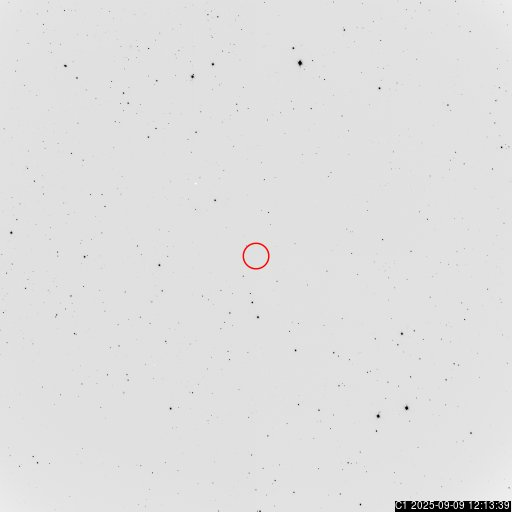
\includegraphics[width=0.65\linewidth]{figure/C1.jpg}

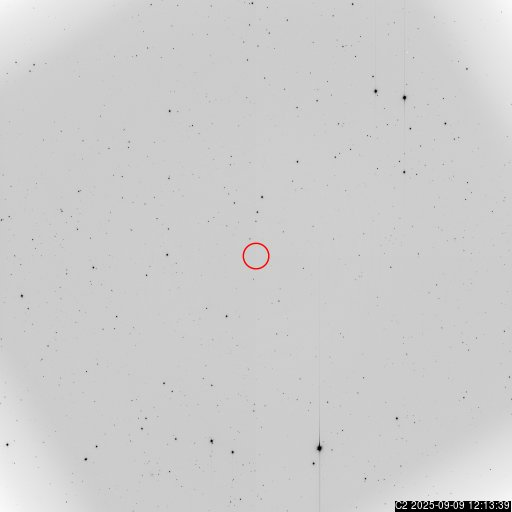
\includegraphics[width=0.65\linewidth]{figure/C2.jpg}

\caption{Typical images in the blue channel (above) and red channel (below). Note that the red channel is flipped vertically with respect to the blue channel because of the reflection off the second dichroic. Note also the vignetting in the red channel caused by the incorrect orientation of the filters and the trails above and below bright stars.}
\label{figure:typical-images}
\end{figure}

\begin{itemize}

\item 
The blue channel is operational and works as expected. 

\item 
The red channel is operation and works largely as expected. However:

\begin{itemize}
    \item Compared to the blue CCD, the red CCD shows worse artifacts above and below bright sources, and we anticipate working with the vendor to tune the CCD voltages and improve this.
    \item There is vignetting in the corners of the red CCD as the filter wheel has an incorrect rotation. We hope to correct this in November 2025.
\end{itemize}

Both of these problems can be seen in Figure~\ref{figure:typical-images}.

\item 
The telescope is operational and working largely as expected. However: 

\begin{itemize}
    \item We have not completed optical alignment of the telescope. As a result of this, we see field-depended comma in both detectors. Nevertheless, the instrument has given images with FWHM of 0.8 arcsec in the center of the field, but the FWHM is worse away from the field center. We hope to complete alignment in November 2025.
    \item The telescope tracking is not as good as we anticipated; although short exposures often have a FWHM of less than 1.0 arcsec, exposures of sixty seconds typically have a FWHM of about 1.2 arcsec. We will work in September 2025 to improve the pointing map and hence the tracking.
\end{itemize}

\item
The automatic data-processing pipeline is not yet available. We still do not have a date for when it will be available. 

However, we have an engineering pipeline that is capable of stacking images and doing a simple sky subtraction. It requires some manual tuning (selecting a star for alignment and determining the fraction of frames to reject). It does not perform astrometric or photometric calibration or produce source catalogs. If you are interested in this pipeline, please contact Alan Watson <\href{mailto:alan@astro.unam.mx}{alan@astro.unam.mx}> directly.

\item
The scheduler is not yet fully integrated. Observations have to be programmed by hand, which limits flexibility and favors blocks that are simpler to program.

\end{itemize}
